% !TEX TS-program = xelatex
% !BIB program = bibtex
% !TeX spellcheck = ru_RU
% !TEX root = talk.tex

\documentclass
  [ russian
  , aspectratio=169 % Для защит онлайн лучше использовать разрешение не 4х3
  ] {beamer}

%%% Обязательные пакеты
%% Beamer
\usepackage{beamerthemesplit}
\usetheme{SPbGU}
\beamertemplatenavigationsymbolsempty
\usepackage{appendixnumberbeamer}

%% Локализация
\usepackage{fontspec}
\setmainfont{CMU Serif}
\setsansfont{CMU Sans Serif}
\setmonofont{CMU Typewriter Text}
%\setmonofont{Fira Code}[Contextuals=Alternate,Scale=0.9]
%\setmonofont{Inconsolata}
% \newfontfamily\cyrillicfont{CMU Serif}

\usepackage{polyglossia}
\setdefaultlanguage{russian}
\setotherlanguage{english}
\usepackage[autostyle]{csquotes} % Правильные кавычки в зависимости от языка

%% Графика
\usepackage{wrapfig} % Позволяет вставлять графику, обтекаемую текстом
\usepackage{pdfpages} % Позволяет вставлять многостраничные pdf документы в текст

%% Математика
\usepackage{amsmath, amsfonts, amssymb, amsthm, mathtools} % "Адекватная" работа с математикой в LaTeX

% Математические окружения с русским названием
\newtheorem{rutheorem}{Теорема}
\newtheorem{ruproof}{Доказательство}
\newtheorem{rudefinition}{Определение}
\newtheorem{rulemma}{Лемма}

%%% Дополнительные пакеты. Используются в презентации, но могут быть отключены при необходимости
\usepackage{tikz} % Мощный пакет для создание рисунков, однако может очень сильно замедлять компиляцию
\usetikzlibrary{decorations.pathreplacing,calc,shapes,positioning,tikzmark}

\usepackage{multirow} % Ячейка занимающая несколько строк в таблице

%% Пакеты для оформления алгоритмов на псевдокоде
\usepackage[noend]{algpseudocode}
\usepackage{algorithm}
\usepackage{algorithmicx}

\usepackage{fancyvrb}

\NewDocumentCommand{\xxHash}{}{\textsc{xxHash}}
\NewDocumentCommand{\riscv}{}{\textsc{RISC-V}}
\NewDocumentCommand{\xxh}{m}{\textsc{XXH{#1}}}
\NewDocumentCommand{\sew}{}{\textsc{SEW}}
\NewDocumentCommand{\vl}{}{\textsc{VL}}
\NewDocumentCommand{\rvv}{}{\textsc{RVV}}
\usepackage{booktabs}
\usepackage{tabularx}
\usepackage{siunitx} % для таблиц с единицами измерений

\setbeamertemplate{itemize items}[circle]
\setbeamertemplate{enumerate items}[circle]

\newcommand\blfootnote[1]{%
	\begingroup
	\renewcommand\thefootnote{}\footnote{#1}%
	\addtocounter{footnote}{-1}%
	\endgroup
}

\makeatletter

\input{pretitle.tex}
\input{title.tex}

\newcommand{\academicGroup}{\my@title@group@ru}
\newcommand{\advisorChair}{\my@title@chair@ru}
% То, что в квадратных скобках, отображается внизу по центру каждого слайда.
\title[Lamagraph: Транслятор в Interaction Nets]{\my@title@title@ru}
% То, что в квадратных скобках, отображается в левом нижнем углу.
\author[\my@title@author@ru]{\my@title@author@ru, группа \academicGroup}
\institute[СПбГУ]{}
\date[25 апреля 2025 г.]{}
\newcommand{\supervisor}{\my@title@supervisor@ru}
\newcommand{\supervisorPosition}{\my@title@supervisorPosition@ru}
\newcommand{\consultant}{\my@title@consultant@ru}
\newcommand{\consultantPosition}{\my@title@consultantPosition@ru}
\newcommand{\reviewer}{\my@title@reviewer@ru}
\newcommand{\reviewerPosition}{\my@title@reviewerPosition@ru}
\newcommand{\defenseYear}{\my@title@year@ru}

\makeatother
\begin{document}
{
\setbeamertemplate{footline}{}
% Лого университета или организации, отображается в шапке титульного листа
\begin{frame}
    \includegraphics[width=1.4cm]{figures/герб_серый.png}
    \vspace{-35pt}
    \hspace{-10pt}
    \begin{center}
        \begin{tabular}{c}
            \scriptsize{Санкт-Петербургский государственный университет} \\
            \scriptsize{\advisorChair}
        \end{tabular}
        \titlepage
    \end{center}

    \btVFill

    {\scriptsize
        % У научного руководителя должна быть указана научная степень
        \textbf{Научный руководитель:}  \supervisorPosition~\supervisor \\
        % Консультанта может и не быть. Должна быть указана должность или ученая степень
        % \textbf{Консультант:}  \consultantPosition~\consultant \\
        % Для учебной практики не обязателен. Должна быть указана должность или ученая степень
        \textbf{Рецензент:} \reviewerPosition~\reviewer \\
        % TODO: добавить условие на включение рецензента в зависимости от вида отчета
    }
    \makeatother
    \begin{center}
        \vspace{5pt}
        \scriptsize{Санкт-Петербург\\ \defenseYear}
    \end{center}
\end{frame}
}

\begin{frame}{Введение}

    \begin{itemize}
        \item Задачи искусственного интеллекта и анализа графов естественным образом выражаются в терминах разреженной линейной алгебры
        \item Разреженная линейная алгебра влечёт за собой нерегулярный параллелизм $\implies$~требуются специализированные ускорители
        \item \INs{}~--- модель вычислений, допускающая параметризацию и в которой легко достигается параллелизм
        \item Существуют программные реализации \INs{}, однако попыток реализовать ускоритель на её основе пока не предпринималось
    \end{itemize}

\end{frame}

\begin{frame}{Interaction Nets}

    \begin{center}
        \includegraphics[width=\textwidth]{figures/in_talk.pdf}
    \end{center}

\end{frame}

\begin{frame}{\Lamagraph{}}

    Проект \Lamagraph{} исследует возможности по разработке
    \begin{itemize}
        \item параметризуемого многоядерного сопроцессора для разреженной линейной алгебры на основе \INs{}
        \item ML-подобного функционального языка для программирования сопроцессора
    \end{itemize}
    \begin{center}
        \includegraphics[width=\linewidth]{figures/lamagraph-big-horiz.pdf}
    \end{center}

\end{frame}

\begin{frame}{Требования к проекту}

    К проекту выдвинуты следующие требования
    \begin{itemize}
        \item Параметризация всех компонентов типами агентов сети и правилами их редукции
        \item Возможность сбора статистики
        \item Возможность постановки сравнительных экспериментов
        \item Использование единого стека технологий~--- гомогенность
        \item Получение полнофункционального прототипа, содержащего все компоненты, важнее, чем детальная проработка какого-то отдельного компонента
        \item Расширяемость и модифицируемость
    \end{itemize}

\end{frame}

\begin{frame}
    \frametitle{Постановка задачи}

    \textbf{Целью} работы является разработка транслятора модельного функционального языка в \INs{}
    \vspace{1em}

    \textbf{Задачи}:
    \begin{enumerate}
        \item Реализовать интерпретатор модельного ML-подобного языка
              \begin{enumerate}
                  \item Конкретный синтаксис языка
                  \item AST и синтаксический анализатор
                  \item Алгоритм вывода типов
                  \item Рассахаривание в обогащенное $\lambda$-исчисление
                  \item Интерпретатор обогащенного $\lambda$-исчисления
              \end{enumerate}
        \item Реализовать интерпретатор \INs{}
        \item Реализовать транслятор из обогащенного $\lambda$-исчисления в \INs{}
    \end{enumerate}

\end{frame}

\begin{frame}
    \frametitle{Архитектура проекта}

    \begin{center}
        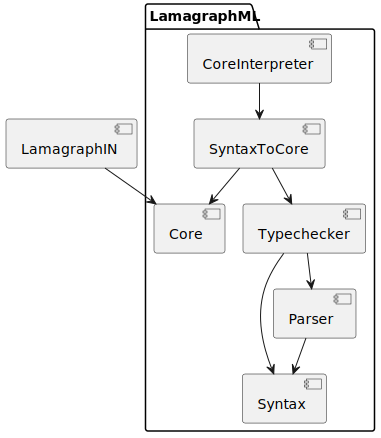
\includegraphics[width=\linewidth]{figures/components.pdf}
    \end{center}

\end{frame}

\begin{frame}{Интерпретатор LamagraphML}

    % \begin{columns}
    % \begin{column}{0.6\textwidth}
    \begin{itemize}
        \item Интерпретатор реализован на \Haskell{}
        \item Используется ML-подобный синтаксис, для представления AST используется паттерн Trees That Grow
        \item Парсер реализован с помощью связки \textsc{Alex} и \textsc{Happy} с применением property-based тестов
        \item Используется система типов Хиндли-Милнера
        \item Для упрощения дальнейших преобразований используется промежуточное представление~--- обогащенное $\lambda$-исчисление
              % \item Для всех компонент применяются golden тесты
    \end{itemize}
    %     \end{column}
    %     \begin{column}{0.35\textwidth}
    %         \begin{center}
    %             \includegraphics[width=\linewidth]{figures/components_compiler.pdf}
    %         \end{center}
    %     \end{column}
    % \end{columns}

\end{frame}

\begin{frame}
    \frametitle{Интерпретатор \INs{}}

    \begin{center}
        \begin{tabular}{lccc}
            \toprule
            \multicolumn{1}{c}{Вид представления}
             & \multicolumn{1}{p{2.5cm}}{\raggedright Удобно для\newline теоретических исследований}
             & \multicolumn{1}{p{2.5cm}}{\raggedright \enquote{Удобно} для реализации на \Haskell{}}
             & \multicolumn{1}{p{2.1cm}}{\raggedright Существует абстрактная машина}                                              \\
            \midrule
            Графовое представление
             & $+$
             & $-$
             & $-$                                                                                                                \\
            Текстовое представление\footnote[frame]{Fernández, Maribel, and Ian Mackie. "A calculus for interaction nets.", 1999}
             & $-$
             & $+$
             & $+$\footnote[frame]{Pinto, Jorge Sousa. "Sequential and concurrent abstract machines for interaction nets.", 2000} \\
            \bottomrule
        \end{tabular}
    \end{center}

    \vspace{1em}

    Таким образом была реализована абстрактная машина Pinto

\end{frame}

\begin{frame}
    \frametitle{Транслятор обогащенного $\lambda$-исчисления в \INs{}}

    \begin{itemize}
        \item \INs{} всё ещё сильно теоретическая область $\implies$ схемы трансляции оперируют чистым $\lambda$-исчислением
        \item Поэтому на данном этапе реализована поддержка только чистого $\lambda$-исчисления
        \item Расширения схемы трансляции для поддержки более широкого класса выражений входного языка~--- предмет дальнейшей работы
    \end{itemize}

\end{frame}

\begin{frame}
    \frametitle{Текущие возможности}

    \begin{center}
        \begin{tabular}{ll}
            \toprule
            Компонент                 & Степень реализации                                \\
            \midrule
            Парсер                    & Реализован полностью                              \\
            Вывод типов               & Нет поддержки алгебраических типов данных         \\
            Рассахаривание            & Поддерживаются только простые паттерны            \\
            Интерпретатор LamagraphML & Нет поддержки взаимной рекурсии                   \\
            Транслятор в \INs{}       & Поддерживается только чистое $\lambda$-исчисление \\
            Абстрактная машина        & Реализована полностью                             \\
            \bottomrule
        \end{tabular}
    \end{center}

\end{frame}

\begin{frame}
    \frametitle{Использование}

    \begin{center}
        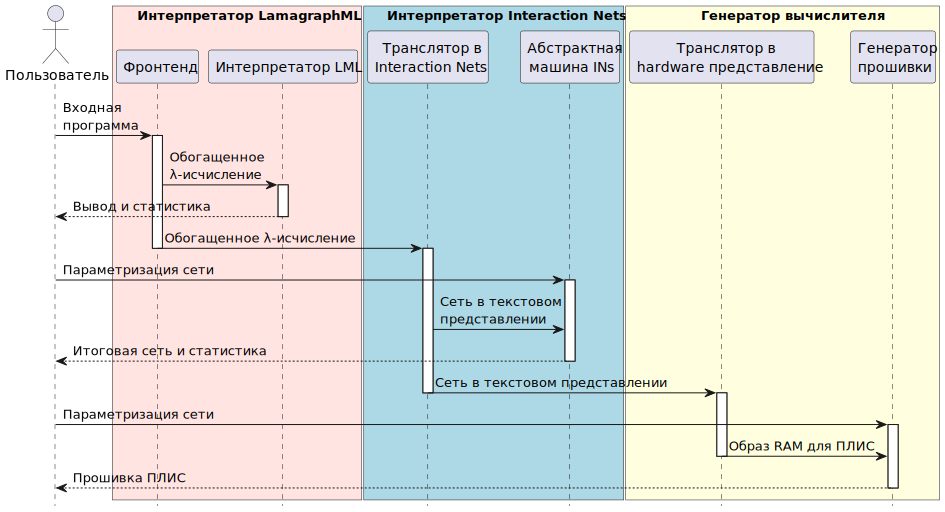
\includegraphics[width=0.8\linewidth]{figures/using.pdf}
    \end{center}

\end{frame}

\begin{frame}
    \frametitle{Пример использования}

    Здесь что-то типа: Мы начали от программы на LML, потом получили из него Core и результат интерпретации (+ счётчики?); из Core перегнали в INs, интерпретировали сеть, получили какой-то терм и счётчики

    Хорошо бы, чтобы счётчики по сетям бились с процессором

\end{frame}

\begin{frame}
    \frametitle{Результаты}
    В рамках производственной практики были достигнуты следующие результаты
    \begin{enumerate}
        \item Реализован интерпретатор модельного ML-подобного языка
        \item Реализован интерпретатор \INs{}
        \item Реализован транслятор из обогащенного $\lambda$-исчисления в \INs{}
    \end{enumerate}

    \vspace{1em}

    Исходный код находится в репозитории: \url{https://github.com/Lamagraph/interaction-nets-in-fpga}

    Имя коммитера: \texttt{WoWaster}
\end{frame}

\end{document}
